\section{Framework Design and Implementation}

\begin{figure}[htp]
  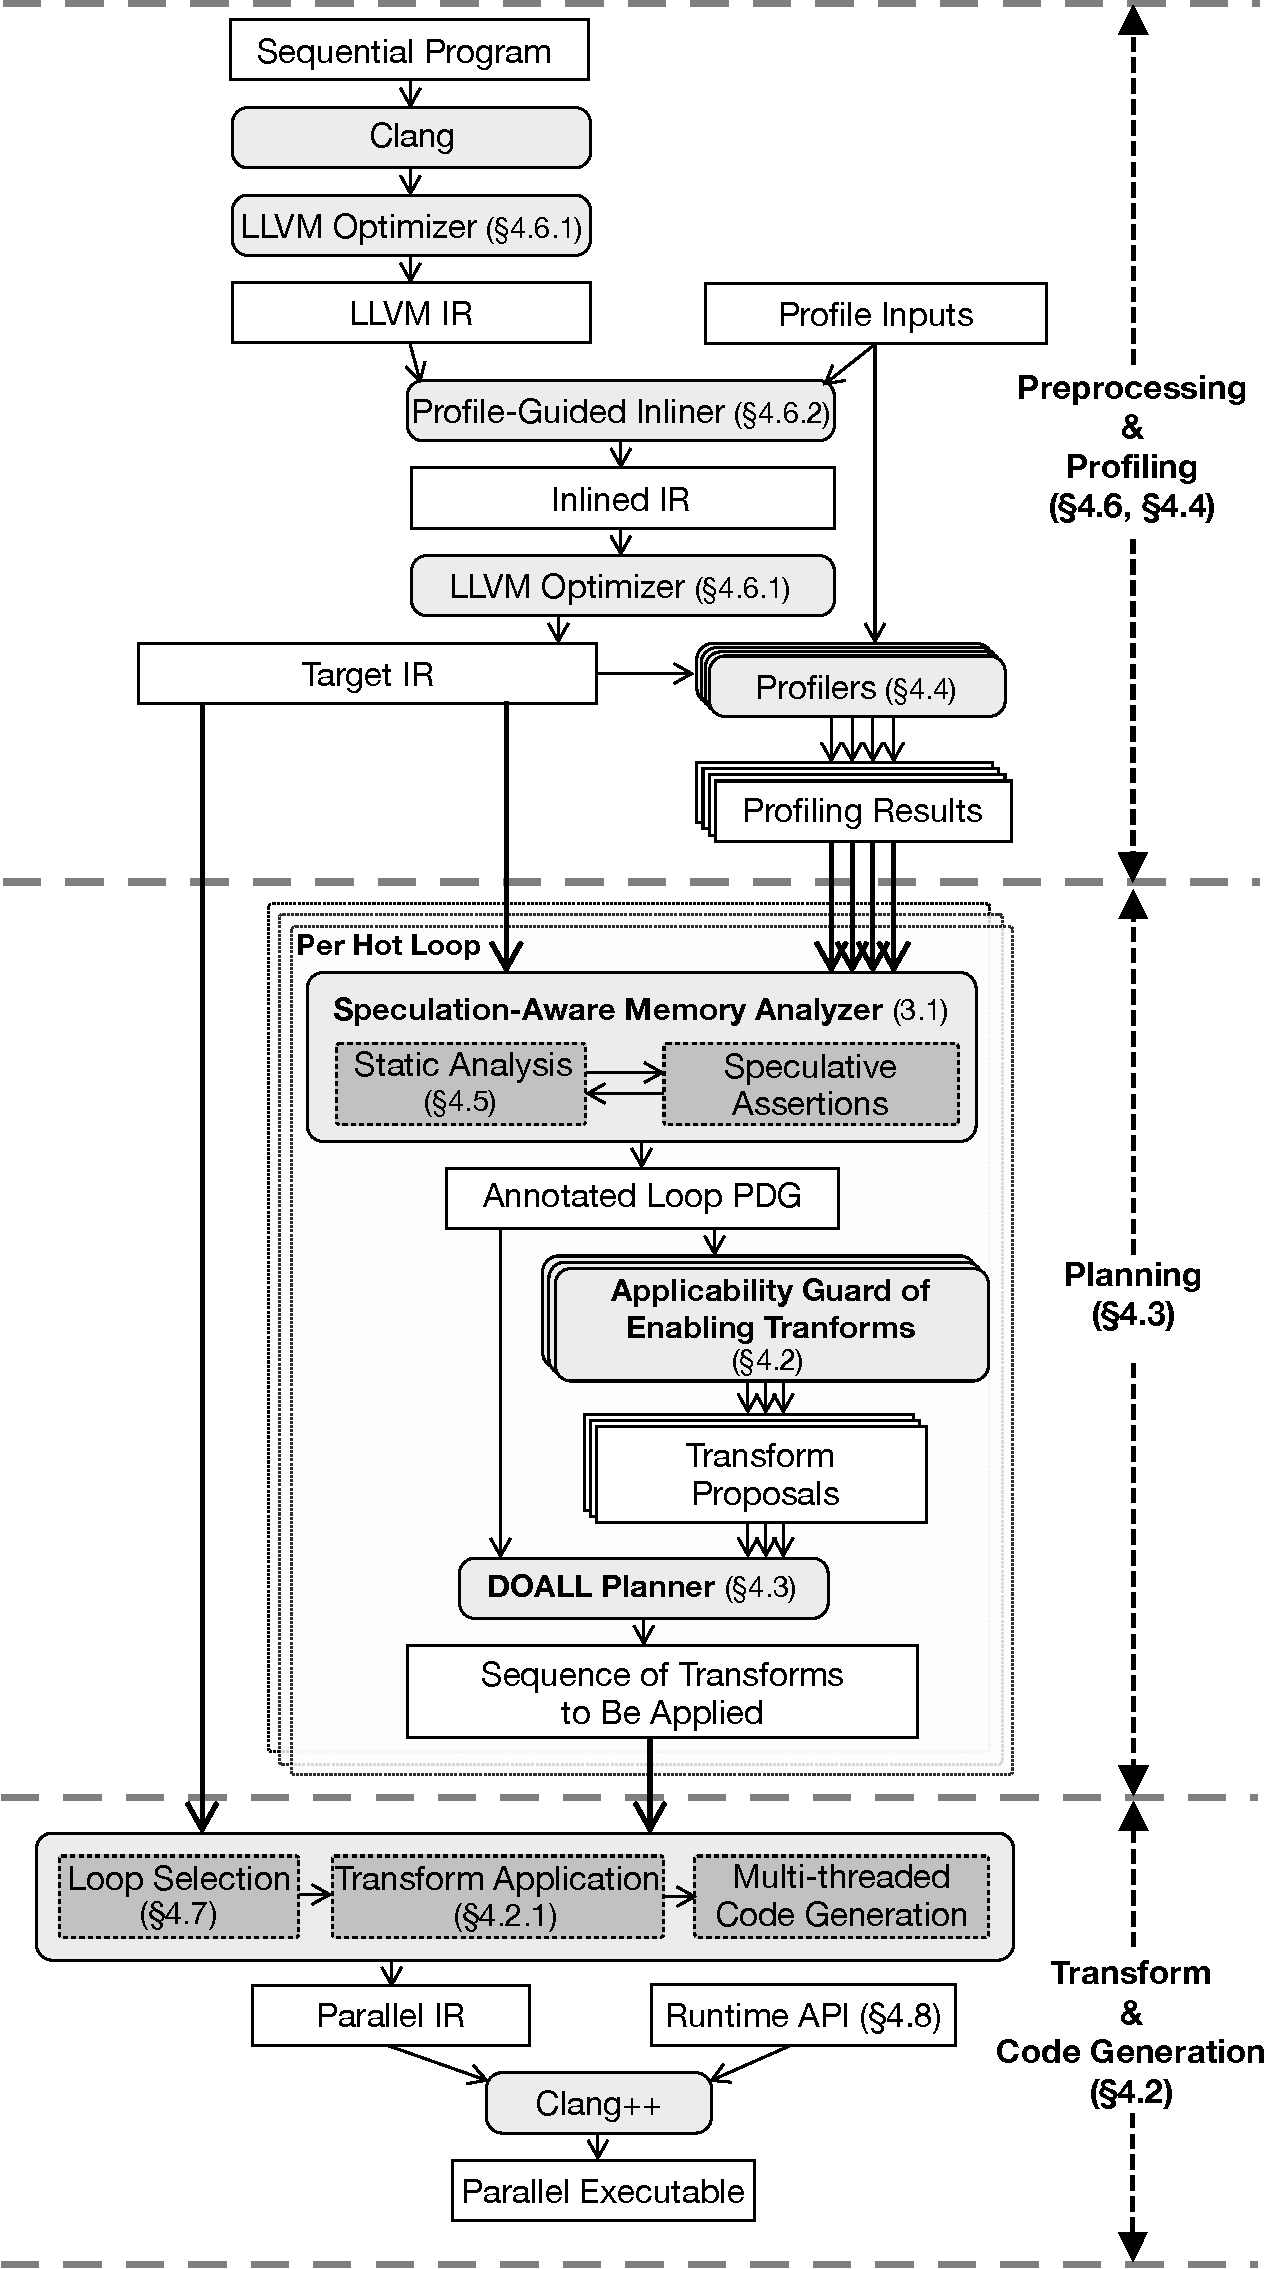
\includegraphics[width=\columnwidth]{figures/compiler-pipeline-crop}
  \caption{\name Framework Overview}
  \label{fig:compiler-pipeline}
\end{figure}

%\name enables efficient speculative parallelization by leveraging
%fine-grained combination of static analysis and cheap-to-validate
%assumptions.
%
Figure~\ref{fig:compiler-pipeline} depicts an overview of the \name
framework, which includes a set of profilers, a parallelizing compiler
and a runtime system.

Initially, the sequential program goes through a few preprocessing
steps and is eventually compiled to a target LLVM intermediate
representation (IR) which is then used to generate profiling results.
Based on profiling results, a set of hot loops is selected.  In the
second phase of the compilation, each hot loop is processed
separately.  The speculation-aware memory analyzer is queried to
annotate a PDG with properties regarding dependences and instructions.
The applicability guards of the enabling transformations examine the
PDG and create transformation proposals to remove
parallelization-inhibiting cross-iteration dependences in the loop. A
DOALL planner considers these proposals, selects the minimum cost
options and generates a sequence of transformations if a profitable
DOALL plan is available.  Finally, we select a set of compatible
parallelizable loops with the maximum profit, apply the tranformations
in their plans, and generate the parallel IR which is then linked with
an runtime and compiled as the parallel executable.

\subsection{Preprocessing}

The compilation process begins with a preprocessing step that
generates the targeted for parallelization intermediate representation
(IR) of the program. We use Clang~\cite{} to generate LLVM~\cite{} IR
from the sequential C/C++ programs followed by LLVM IR optimizations.
Then we perform a pass of profile-guided aggressive, yet selective
inlining and finally another round of LLVM IR optimizations to produce
the target LLVM IR that is used as the starting point for the rest of
the compilation process.

\subsubsection{Clang and LLVM optimizations}

Transformations in this preprocessing step are crucial for the
applicability and profitability of parallelization.
%
Parallelizing compilers usually just compile the source code with -O3
flag to get an initial IR version and then perform a few additional
passes.
%
However, traditional compiler transformations are meant for optimized
sequential execution.
%
Some of these optimizations could unnecessarily complicate the code
and block parallelization efforts.
%
Any performance improvements from these optimizations are negligible
compared to the benefits of successful parallelization.
%
For example, LLVM tries to sink common instructions from two different
execution paths. This reduces the code size but when applied to memory
operations, it complicates the inference of the underlying objects.
%
To avoid such problems, \namensp 's preprocessing step only applies a
small set of LLVM IR enabling transformations that simplify and
canonicalize the IR.

Contrary to LLVM IR optimizations, frontend optimizations by Clang can
be applied more freely.
%
If Clang optimizations are not applied then some information extracted
from the source code could be omitted from the generated LLVM IR.  In
fact, we noticed that when no optimization is used in the frontend
(\textit{clang -O0 -Xclang -disable-O0-optnone}), some very helpful
LLVM intrinsics (e.g., lifetime start/end intrinsics for stack
allocations) are lost.  To avoid this, we compile with -O1 flag for
frontend optimizations but disable LLVM optimizations (\textit{-O1
-Xclang -disable-llvm-passes}).


\subsubsection{Profile-Guided Selective Inlining}

Interprocedural analysis is complicated and expensive, restricting the
precision or scalability of static analysis.
%
Dependences related to callsites often prevent parallelization or lead
to extensive usage of expensive-to-validate memory flow speculation.
%
Inlining can mitigate this problem, but the heuristics used in
industrial compilers are tailored for sequential execution
optimization and are mostly irrelevant to effective parallelization.
%
% code size expansion
%When parallelization is applicable, these
%
More aggressive inlining is needed for parallelization. Naive
aggressive inlining, though, would lead to code size explosion and
exponential increase in compilation time. Avoiding inlining in some
cases
%Filtering of some callsites
is still essential.
%

\name uses profile information to detect hot loops and speculatively
dead callsites.  Only callsites that are within these hot loops and
that cannot be speculated away with control speculation are inlined.
%
Of these callsites, \name also avoids inlining the ones that do not
sink or source cross-iteration dependences that inhibit DOALL
parallelization.
%
%just get a summary.  hard to handle them separetely end up
%overspeculating because it is hard to find the problem.

Inlining is sometimes also useful outside the hot loops.
%
Static analysis can easily infer alias and underlying object queries
for global variables whose address is never
captured~\cite{johnson:17:cgo}.  However, if the address of a global
variable is passed as an argument to a function, then the analysis in
most cases conservatively assumes that the address is stored in memory
(i.e. captured)  within the function. Inlining diminishes this
pproblem.

\subsection{Profiling}
%\subsection{Speculative Assumptions}

A set of profilers generate speculative assumptions:
%
(i) an edge profiler~\ref{llvm_edge_profiling} identifies biased
branches and produces a speculative control flow that can be used by
analysis passes, or directly disprove dependences on speculatively
dead basic blocks;
%
(ii) a memory flow dependence  profiler (\`{a} la
~\cite{privateer4citation}) asserts absence of non-observed data
flows;
%
(iii) a value-prediction profiler (\`{a} la
~\cite{privateer11citation}) detects predictable loads;
%
(iv) a pointer-to-object profiler (\`{a} la ~\cite{johnson:12:pldi})
produces a points-to map that allows detection of underlying objects
for every memory access; and,
%
(v) an object lifetime profiler (\`{a} la ~\cite{johnson:12:pldi})
detects short-lived memory objects, namely objects that exist only within a
single loop iteration.
%

\subsection {Static Analysis}
\name uses a state-of-the-art memory dependence analysis framework
tailored for parallelization (\`{a} la CAF\cite{johnson:14:pldi}), in
which multiple simple analysis algorithms collaboratively attempt to
disprove dependences and minimize the need for speculation.
%
% Static analysis is also used to identify underlying memory objects of
% memory operations and characterize dependences that cannot
% be disproved (see section~\ref{overview_dependence_analysis}).
%In section~\ref{} we discussed how a dependence is characterized as
%\textit{overwrite}.

\paragraph{Extended Kill-Flow Analysis Algorithm:}
%\paragraph{Static Analysis Improvement}
Kill-Flow is a highly effective analysis algorithm that searches for
killing operations along all feasible paths between two operations. If
a killing operation is found, then these two operations cannot have a
dependence.  Since  there  may  be  infinitely  many  paths,  its
search is restricted to blocks which post-dominate the source of the
queried dependence and dominate the destination.
%
This approximation prevents detection of a common pattern (seen in
052.alvinn, 179.art, dijkstra) that can be observed in the code in
Figure~\ref{fig:dijkstra_motivation}.
%
The write to \texttt{\textbf{pathcost}} in line \textbf{29} kills
values flowing from the previous iteration to the read in line \textbf{41}.
However, there is no dominance
relation, and thus it cannot be detected.
%
We extend the Kill-Flow algorithm to detect this pattern. Observe that
the loop header of the inner loop in line \textbf{28} dominates the
read in line \textbf{41}. The extended Kill-Flow treats this inner loop as a single
operation that overwrites a range of memory locations. This way, it
can easily be proven that this range write overwrites
the memory addresses that are read in line \textbf{41} at every iteration.
%
%The effect of this extension on the running time of Kill-Flow is
%negligible.
%
This extension allows us to disprove additional data flows compared to
the state-of-the-art and further reduce the need for memory
speculation.


\subsection{Enabling Transformations}
\label{design_transf}
Enabling transformations address memory, register or/and control
cross-iteration dependences.

\subsubsection{Memory Dependences}

Memory-related enabling transformation collect a set of memory objects
for which they are applicable (see ~\ref{enablers}).

%TODO: maybe add discussion about their cost

\begin{itemize}
%
\item Privatization: Discussed in ~\ref{novel_transf}

\item Reduction: Applicable for objects that only participate to
reduction operations. When applied, separates its objects to the
reduction heap and inserts separation checks (check that their
accesses are within this heap). During runtime, separation is checked
and at commit objects of parallel workers are
merged according to their reduction operation.

%Applicability guard: objects that only participate to reduction
%operations

%Transformation Application: only separate objects to reduction heap

%Runtime support: at commit merge all objects according to their
%reduction operation

\item Short-lived: Applicable for objects that only exist within one
iteration of the loop. When applied, separates its objects to the
short-lived heap and inserts check to ensure separation and that all
the objects of the heap are freed at the end of the iteration. During
runtime, the short-lived property and separation are checked.

\item Read-only: Applicable for objects that are never written to.
When applied, separates its objects to the read heap and inserts
separation checks.  During runtime, separation is checked.

\item TXIO: Applicable for shared IO objects. When applied, it
replaces IO library calls with custom calls. During runtime, it
collects output operations and performs them in order at commit.

\end{itemize}

\subsubsection{Register \& Control Dependences}

Cross-iteration register dependences
%(not related to induction variables)
are handled with reduction, replication, control speculation or value
prediction. Replication replicates side-effect free computation across
parallel workers to overcome cross-iteration dependences and avoid
inter-thread communication.
%
Cross-iteration control dependences are handled either with
replication or control speculation.
%mention IV?
Use of replication allows handling of uncounted loops, namely loops
with unknown trip count when the loop is invoked.
%
In terms of transformation cost, all transformations have constant
cost except for replication.  Replication's cost depends on how many
instructions need to be replicated. Non-speculative enablers
(reduction and replication) are preferred, in most cases, over
speculative ones, and reduction is preferred over replication.

%Cross-iteration register and control dependences related to induction
%variables are handled differently if detected.

%handling live-outs, loop-carried
%
%In the case of speculative executive, registers with cross-iteration
%dependences and live-out registers
%are stored in memory at commit so that they are recoverable in case of
%misspeculation. For live-outs, storing to memory

%\begin{itemize}
%
%\item Scalar Reduction
%
%\item Replication: Replicate side-effect free computation across
%parallel workers.
%
%\end{itemize}
%
%\subsubsection{Control Dependences}
%
%\item Induction Variable Detection: Every worker gets assigned a
%
%\item Replication: Replicate cross-iteration control dependences for
%each worker
%
%\item Control Speculation: Speculate cross-iteration control
%dependences


\subsection{Loop Selection} An execution time profiler, similar to
gprof~\cite{Privateer26}, finds hot loops (at least 10\% of total
program execution).
%
For each hot loop, the compiler finds a DOALL parallelization plan and
estimates its profitability.
%
Out of the profitably parallelizable loops, certain loops are not
selected for parallelization. The excluded loops are either
simultaneously active with another more profitable loop (we do not
support nested parallelism) or their memory object assignments
conflict with the assignments of a more profitable loop (every memory
object can be allocated to only one heap throughout the program in our
current implementation).

\subsection{Runtime}
\subsection{Runtime}
% XXX Maybe a better word than universal. Want to highlight that it handles
% both spec and non-spec

\name provides an efficient runtime
for both speculative and non-speculatively parallelized programs.

% Process-based approach gives us:
%   1. Cheap live-in copying
%   2. Separation between speculative and committed state
%   3. Cheap heap checks
\paragraph{Process-based approach}
The runtime system of \name uses a process-based parallelization scheme,
as opposed to a thread-based one for multiple reasons. First, it allows the
use of copy-on-write (CoW) semantics of
processes to achieve low overhead for communicating live-in values from the
main process to the workers.
% Or do we force it to use CoW?
It also gives an implicit separation between the speculative states of the
workers and the committed state that the main process sees when
speculation is used. To facilitate cheap heap assignment validation, we
segment each worker's virtual memory address into disjoint sections,
corresponding to each transform's heap, enabling cheap heap assignment
checks.
% which heap an object
% belongs to becomes trivial, involving only a bitwise \texttt{AND} of the
% object's virtual address with its heap's address mask.
% This segmentation
% also gives an added benefit of reducing the overhead for logging, as
% This is not possible
% with a thread-based system, in which workers share the same virtual address
% space.

% Shared is used for checkpointing, copying live-outs, and independently
% privatized objects. Although the runtime code uses shared memory for
% other purposes (private, redux, shadow), this is only an implementation
% detail that makes the code more readable.
\paragraph{Use of shared memory}
We utilize POSIX named shared memory in \texttt{\textbf{/dev/shm}} to share
data among workers and the main process.
% Do we explain what independently privatized means?
For non-speculatively parallelization plans, we can use
\texttt{\textbf{mmap()}} with shared permissions,
% to share the independent heap
% from the main process, which
negating the overhead of merging worker states and copying out live-out values.
% To avoid the cost of multiple forks() at runtime, we spawn processes only
% once at the beginning of the program and remap each worker's virtual memory
% at the start of each invocation.
To avoid the overhead of process spawning for inner loops with multiple
invocations (\texttt{052.alvinn}), we \texttt{\textbf{fork()}} only once at
program startup and remap each worker's virtual memory at the start of
every invocation.
% For inner loops with multiple invocations (parallelized loop in
% \texttt{052.alvinn}), we \texttt{\textbf{fork()}} only once at the
% beginning
% at every invocation and remap each worker's virtual memory at the start
% of every invocation.
% This gives us performance near that of
% thread-based systems for non-speculative (independent) privatization.
% Shared memory is also used for collecting each worker's private memory
% during a checkpoint operation. The last worker to reach a checkpoi
% Does not integrate well with the previous sentence

% \paragraph{Logging and validation}
% Each transformation inserts specialized logging and validation for the
% objects that it handles; depending on the transformation, these checks may
% trigger misspeculation. Note that these checks only detects disallowed
% operations within iterations of each worker, and not across workers.

\paragraph{Checkpointing and misspeculation}
Checkpointing is used to validate reads and writes to private objects
across workers and save the current program state in
the case of misspeculation. When a worker reaches an iteration marked with
a checkpoint operation, it will map the checkpoint object to its virtual
memory space and ensure that its own writes to privatized data did not
coincide with a read by another worker.
% Checkpointing is inherently
% sequential and increasing the amount of data that needs to be merged can
% significantly affect the overall performance.

\paragraph{Recovery}
The use of speculation necessitates recovery code in case
misspeculation occurs.
When misspeculation is detected by a worker, either during an
iteration or at checkpoint time, other workers continue up to and commit the last
valid checkpoint, then wait for recovery to finish.
The main process will execute the loop
sequentially up to and including the misspeculated iteration, using the
committed checkpoint as the starting state, and restart the parallel
workers.
% Restarting
% the workers at this point is no different from beginning the invocation,
% aside from the starting iteration sent to the workers.


%In this work, we introduce a set of transformations to explore more
%opportunities of parallelization.
%
%%We call these enabling transformations Enablers.
%
%%  How to query Enabler?
%
%One thing that hinders these Enablers from working coordinately is
%the phase-ordering problem, which means one transformation could be disabled
%by a previous transformation. Another problem is the increasing
%implementation and maintainance difficulty when more and more Enablers are
%put in the framework. To avoid these problems, we carefully organize the
%framework in a way that all Enablers are modular and independent. As a first
%step, all loop-carried dependences are identified by the frontend and passed
%to each Enabler, who tries to address each dependence by its best effort and
%returns a remedy along with the cost if a way to remove the dependence is
%available. If all dependences are removable by at least one Enablers, the
%parallel code generation part will choose the remedy with the lowest cost
%for each dependence and generate the parallel binary. This scheme seperates
%the desicion part from the actual transformation and allows us to evaluate
%the cost of each dependence separetely and choose the most profitable plan
%instead of applying all transformations in a fixed order. For simplicity, we
%assigned to each Enabler a predefined cost in this work. Yet in Table.
%\ref{table:enabler-stats}, we provided the statistics of the applicable and
%chosen Enabler to show how this framework makes the tradeoff when more than
%one Enablers are available. This study is not available for a traditional
%approach of transformations.
%
%The analysis passes and the transformation passes are seperated. Even though
%it has been suggested before, in this work, we have a smaller set of
%Enablers with stronger capability.

%\textbf{Non-Speculative Transformations}
%
%\begin{itemize}
%    \item Conservative Reduction (ReduxRemed)
%        % Both scalar and memory reduction
%
%    \item Conservative Privatization (PrivRemed)
%        % Removes loop-carried false memory dependences on conservatively provable privitizable objects
%
%    \item Memory Versioning (MemVerRemed)
%        % Assumes privatized memory for each thread
%        % Removes loop-carried false memory dependences
%        % Stronger but more expensive than PrivRemed
%        % Process-based parallelization enforces this remediator
%
%    % \item Counted Loop Detection (CountedIVRemed)
%        % Removes loop-carried register and control dependences related to induction variables on counted loops
%
%    \item TXIO (TXIORemed)
%        % I/O deferral
%        % Delays execution of instructions with side-effects, such as I/O operations
%
%    % \item Conservative Loop Fission (LoopFissionRemed) ???
%        % Separate non-DOALL SCCs to an initial sequential stage (loop in this case)
%        % Only small sequential stages considered
%        % No usage of speculative remediators to achieve separation
%\end{itemize}
%
%\textbf{Speculative Transformations}
%
%\begin{itemize}
%    \item Control Speculation (ControlSpecRemed)
%        % Based on edge profile info, removes control flow edges and considers all basic blocks dominated by these edges as speculatively dead
%        % Inexpensive runtime validation
%
%    \item Value Prediction (LoadedValuePred)
%        % Some load instructions always read a single, predictable value from memory
%        % Loop-Invariant Loaded-Value
%        % Inexpensive runtime validation
%
%    \item Header-phi prediction (HeaderPhiPredRemed)
%        % Some phi instructions have a predictable value.
%        % Allows removal of loop-carried register dependeces
%        % Inexpensive runtime validation
%
%    \item Separation Speculation (LocalityRemed)
%
%        % Johnson et al. PLDI '12
%
%        % Separation speculation partitions a program's allocations into a few disjoint "families" of objects and speculatively assumes that every pointer in the program refers exclusively to objects in one family. Under this assumption, if two pointers reference distinct families, they cannot alias.
%
%        % Relatively inexpensive runtime validation due to small number of families, allocation of objects in family-specific memory regions, runtime optimizations and thread-local checks (no communication among concurrent threads needed).
%
%        % Secondary speculation built on top of separation speculation:
%
%        %     Read-only speculation
%        %         Read-only family
%        %         Some memory objects are never modified but static dependence analysis is sometimes unable to prove this property
%        %         Objects in the read-only family are only accessed by read-only memory operations. Thus, speculatively read-only memory operations never experience flow, anti or output dependences
%        %         Apart from separation speculation validation, no other validation is required
%
%        %     Speculative accumulator expansion
%        %         Compiler identifies accumulators as values which are repeatedly updated with an associative and commutative operator (a reduction) but whose intermediate values are otherwise unused within the loop. Static dependence sometimes fails to prove that every access to a given storage location is a reduction or that intermediate values are never used.
%        %         The pointer-family assumption establishes that objects in the reduction family are only accessed by load-reduce-store sequences and consequently that intermediate values cannot be otherwise observed or modified.
%        %         Apart from separation speculation validation, no other validation is required
%
%        %     Speculative privatization
%        %         Reuse of data structures with no flow dependences from one iteration to the other prevents parallelization due to anti or output dependences.
%        %         Addressed by having a private copy of the data structure for each iteration
%        %         Assumption: loads from certain private objects never read values stored during earlier iterations of the loop.
%        %         Privatization criteria validated in two phases, one thread-local and one more expensive that requires communication among threads.
%
%        %     Object-lifetime speculation
%        %         Short-lived objects
%        %         Some objects allocated within a loop iteration are always deallocated before the end of that same iteration. Static dependence analysis often fails to identify this case.
%        %         Loads from or stores to such objects cannot depend on memory accesses in other iterations.
%        %         Extra validation on top of separation speculation validation: object lifetime speculation must validate that short-lived objects never outlive their iteration. Thread-local checks.
%
%    \item Memory Flow Speculation (SmtxSlampRemed \& SmtxLampRemed)
%        % Assumes the absence of flow dependences between memory operations when not manifested during profiling.
%        % Provides as much or more an enabling effect than many other types of speculation.
%        % Expensive validation. Requires communication among concurrent threads.
%
%    \item Speculative AA stack (MemSpecAARemed)
%        % Allows collaboration among memory flow speculation, control speculation, value prediction, speculative points-to analysis and static analysis.
%        % Demonstrates the power of collaboration among remediators, and between speculation techniques and static analysis.
%        % Provides at least as much coverage as all the remediators addressing mem deps combined (only excludes SLAMP mem spec and localityaa).
%
%    % \item Speculative Loop Fission (LoopFissionRemed) ???
%        % Same as Conservative Loop Fission apart from the fact that it requires usage of speculative remediators to achieve separation
%
%    \item Pointer-Residue Speculation (PtrResidueRemed)
%        % Never part of a paper. Never evaluated. Idea published in Nick Johnson's thesis
%        % Separation speculation disambiguates references to different objects, but does not disambiguate references within the same object. Pointer-residue speculation works at the sub-object level.
%        % It disambiguates different fields within an object and in some cases recognizes different regular strides across an array.
%        % It characterizes each pointer expression in the program according to the possible values of its four least-significant bits (residue).
%        % Examines whether residue sets are disjoint with respect to the size of the memory accesses of two given operations.
%\end{itemize}
%
%Second Level Enabler
%\begin{itemize}
%    \item Replicable Stage (RepStageRemedy)
%\end{itemize}
%
%\subsection{Enabler Statistics}
% Insert the table here

% 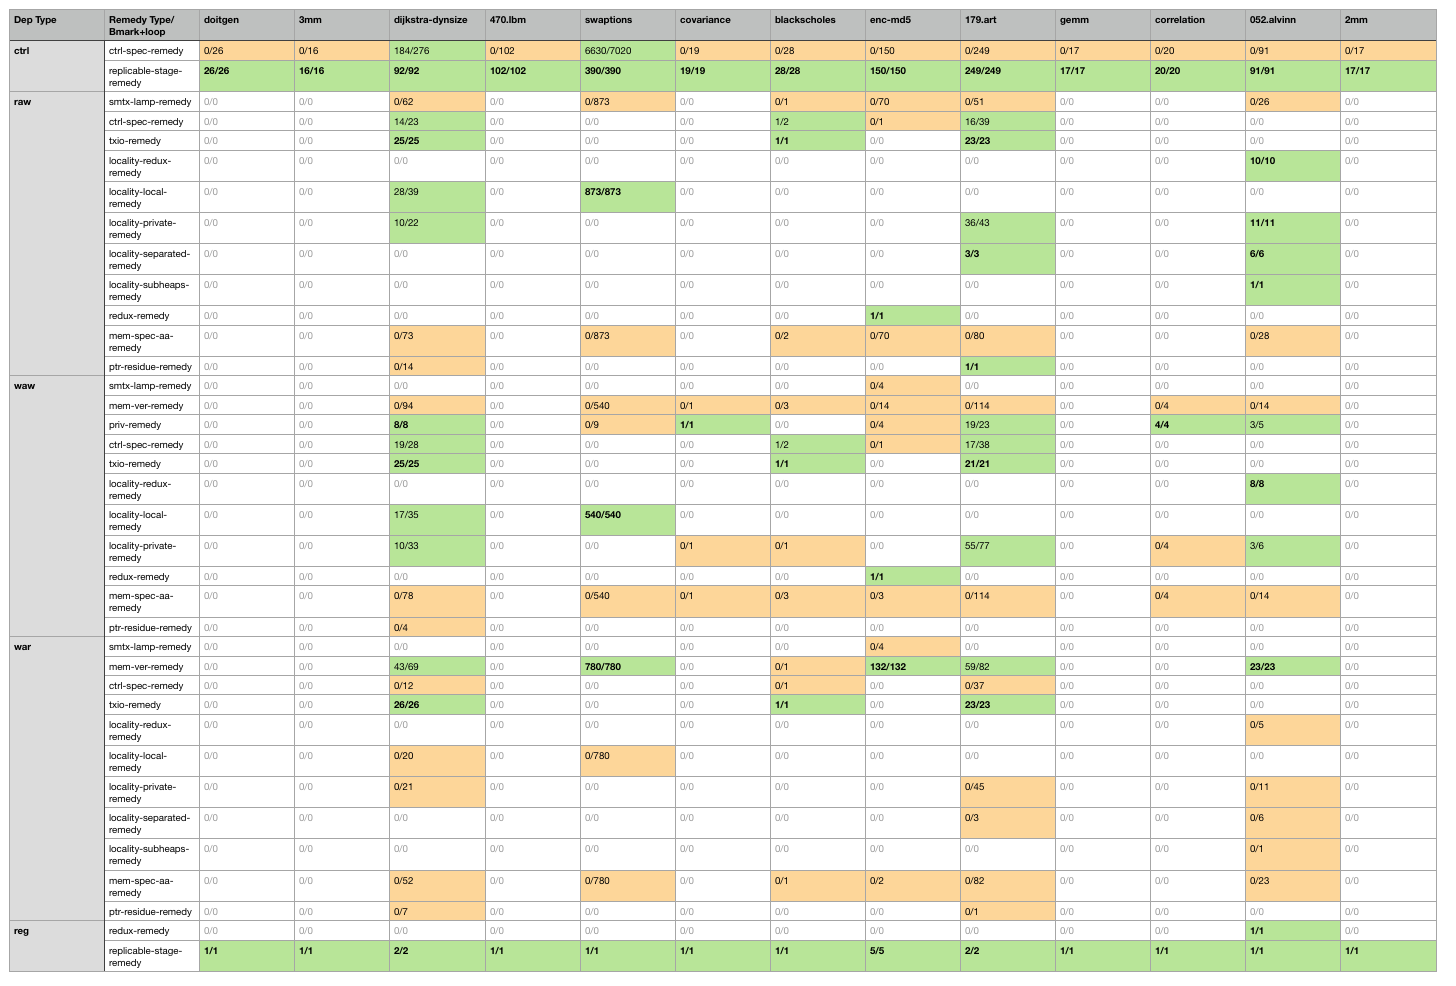
\includegraphics[width=\textwidth]{figures/table.png}
% \label{table:enabler-stats}


% \begin{table}[]
% \label{table:enabler-stats}
% \begin{tabular}{lllllllllllllll}

% Dep Type & Remedy Type/Bmark+loop    & doitgen & 3mm   & dijkstra-dynsize &
% 470.lbm & swaptions & covariance & blackscholes & enc-md5 & 179.art & gemm  &
% correlation & 052.alvinn & 2mm   \\

% ctrl     & ctrl-spec-remedy          & 0/26    & 0/16  & 184/276          &
% 0/102   & 6630/7020 & 0/19       & 0/28         & 0/150   & 0/249   & 0/17  &
% 0/20        & 0/91       & 0/17  \\

%          & replicable-stage-remedy   & 26/26   & 16/16 & 92/92            &
%          102/102 & 390/390   & 19/19      & 28/28        & 150/150 & 249/249 &
%          17/17 & 20/20       & 91/91      & 17/17 \\

% raw      & smtx-lamp-remedy          & 0/0     & 0/0   & 0/62             & 0/0
% & 0/873     & 0/0        & 0/1          & 0/70    & 0/51    & 0/0   & 0/0
% & 0/26       & 0/0   \\
%          & ctrl-spec-remedy          & 0/0     & 0/0   & 14/23            & 0/0
%          & 0/0       & 0/0        & 1/2          & 0/1     & 16/39   & 0/0   &
%          0/0         & 0/0        & 0/0   \\

%          & txio-remedy               & 0/0     & 0/0   & 25/25            & 0/0
%          & 0/0       & 0/0        & 1/1          & 0/0     & 23/23   & 0/0   &
%          0/0         & 0/0        & 0/0   \\

%          & locality-redux-remedy     & 0/0     & 0/0   & 0/0              & 0/0
%          & 0/0       & 0/0        & 0/0          & 0/0     & 0/0     & 0/0   &
%          0/0         & 10/10      & 0/0   \\

%          & locality-local-remedy     & 0/0     & 0/0   & 28/39            & 0/0
%          & 873/873   & 0/0        & 0/0          & 0/0     & 0/0     & 0/0   &
%          0/0         & 0/0        & 0/0   \\

%          & locality-private-remedy   & 0/0     & 0/0   & 10/22            & 0/0
%          & 0/0       & 0/0        & 0/0          & 0/0     & 36/43   & 0/0   &
%          0/0         & 11/11      & 0/0   \\

%          & locality-separated-remedy & 0/0     & 0/0   & 0/0              & 0/0
%          & 0/0       & 0/0        & 0/0          & 0/0     & 3/3     & 0/0   &
%          0/0         & 6/6        & 0/0   \\

%          & locality-subheaps-remedy  & 0/0     & 0/0   & 0/0              & 0/0
%          & 0/0       & 0/0        & 0/0          & 0/0     & 0/0     & 0/0   &
%          0/0         & 1/1        & 0/0   \\

%          & redux-remedy              & 0/0     & 0/0   & 0/0              & 0/0
%          & 0/0       & 0/0        & 0/0          & 1/1     & 0/0     & 0/0   &
%          0/0         & 0/0        & 0/0   \\

%          & mem-spec-aa-remedy        & 0/0     & 0/0   & 0/73             & 0/0
%          & 0/873     & 0/0        & 0/2          & 0/70    & 0/80    & 0/0   &
%          0/0         & 0/28       & 0/0   \\

%          & ptr-residue-remedy        & 0/0     & 0/0   & 0/14             & 0/0
%          & 0/0       & 0/0        & 0/0          & 0/0     & 1/1     & 0/0   &
%          0/0         & 0/0        & 0/0   \\

% waw      & smtx-lamp-remedy          & 0/0     & 0/0   & 0/0              & 0/0
% & 0/0       & 0/0        & 0/0          & 0/4     & 0/0     & 0/0   & 0/0
% & 0/0        & 0/0   \\

%          & mem-ver-remedy            & 0/0     & 0/0   & 0/94             & 0/0
%          & 0/540     & 0/1        & 0/3          & 0/14    & 0/114   & 0/0   &
%          0/4         & 0/14       & 0/0   \\

%          & priv-remedy               & 0/0     & 0/0   & 8/8              & 0/0
%          & 0/9       & 1/1        & 0/0          & 0/4     & 19/23   & 0/0   &
%          4/4         & 3/5        & 0/0   \\

%          & ctrl-spec-remedy          & 0/0     & 0/0   & 19/28            & 0/0
%          & 0/0       & 0/0        & 1/2          & 0/1     & 17/38   & 0/0   &
%          0/0         & 0/0        & 0/0   \\

%          & txio-remedy               & 0/0     & 0/0   & 25/25            & 0/0
%          & 0/0       & 0/0        & 1/1          & 0/0     & 21/21   & 0/0   &
%          0/0         & 0/0        & 0/0   \\

%          & locality-redux-remedy     & 0/0     & 0/0   & 0/0              & 0/0
%          & 0/0       & 0/0        & 0/0          & 0/0     & 0/0     & 0/0   &
%          0/0         & 8/8        & 0/0   \\

%          & locality-local-remedy     & 0/0     & 0/0   & 17/35            & 0/0
%          & 540/540   & 0/0        & 0/0          & 0/0     & 0/0     & 0/0   &
%          0/0         & 0/0        & 0/0   \\

%          & locality-private-remedy   & 0/0     & 0/0   & 10/33            & 0/0
%          & 0/0       & 0/1        & 0/1          & 0/0     & 55/77   & 0/0   &
%          0/4         & 3/6        & 0/0   \\

%          & redux-remedy              & 0/0     & 0/0   & 0/0              & 0/0
%          & 0/0       & 0/0        & 0/0          & 1/1     & 0/0     & 0/0   &
%          0/0         & 0/0        & 0/0   \\

%          & mem-spec-aa-remedy        & 0/0     & 0/0   & 0/78             & 0/0
%          & 0/540     & 0/1        & 0/3          & 0/3     & 0/114   & 0/0   &
%          0/4         & 0/14       & 0/0   \\

%          & ptr-residue-remedy        & 0/0     & 0/0   & 0/4              & 0/0
%          & 0/0       & 0/0        & 0/0          & 0/0     & 0/0     & 0/0   &
%          0/0         & 0/0        & 0/0   \\

% war      & smtx-lamp-remedy          & 0/0     & 0/0   & 0/0              & 0/0
% & 0/0       & 0/0        & 0/0          & 0/4     & 0/0     & 0/0   & 0/0
% & 0/0        & 0/0   \\

%          & mem-ver-remedy            & 0/0     & 0/0   & 43/69            & 0/0
%          & 780/780   & 0/0        & 0/1          & 132/132 & 59/82   & 0/0   &
%          0/0         & 23/23      & 0/0   \\

%          & ctrl-spec-remedy          & 0/0     & 0/0   & 0/12             & 0/0
%          & 0/0       & 0/0        & 0/1          & 0/0     & 0/37    & 0/0   &
%          0/0         & 0/0        & 0/0   \\

%          & txio-remedy               & 0/0     & 0/0   & 26/26            & 0/0
%          & 0/0       & 0/0        & 1/1          & 0/0     & 23/23   & 0/0   &
%          0/0         & 0/0        & 0/0   \\

%          & locality-redux-remedy     & 0/0     & 0/0   & 0/0              & 0/0
%          & 0/0       & 0/0        & 0/0          & 0/0     & 0/0     & 0/0   &
%          0/0         & 0/5        & 0/0   \\

%          & locality-local-remedy     & 0/0     & 0/0   & 0/20             & 0/0
%          & 0/780     & 0/0        & 0/0          & 0/0     & 0/0     & 0/0   &
%          0/0         & 0/0        & 0/0   \\

%          & locality-private-remedy   & 0/0     & 0/0   & 0/21             & 0/0
%          & 0/0       & 0/0        & 0/0          & 0/0     & 0/45    & 0/0   &
%          0/0         & 0/11       & 0/0   \\

%          & locality-separated-remedy & 0/0     & 0/0   & 0/0              & 0/0
%          & 0/0       & 0/0        & 0/0          & 0/0     & 0/3     & 0/0   &
%          0/0         & 0/6        & 0/0   \\

%          & locality-subheaps-remedy  & 0/0     & 0/0   & 0/0              & 0/0
%          & 0/0       & 0/0        & 0/0          & 0/0     & 0/0     & 0/0   &
%          0/0         & 0/1        & 0/0   \\

%          & mem-spec-aa-remedy        & 0/0     & 0/0   & 0/52             & 0/0
%          & 0/780     & 0/0        & 0/1          & 0/2     & 0/82    & 0/0   &
%          0/0         & 0/23       & 0/0   \\

%          & ptr-residue-remedy        & 0/0     & 0/0   & 0/7              & 0/0
%          & 0/0       & 0/0        & 0/0          & 0/0     & 0/1     & 0/0   &
%          0/0         & 0/0        & 0/0   \\

% reg      & redux-remedy              & 0/0     & 0/0   & 0/0              & 0/0
% & 0/0       & 0/0        & 0/0          & 0/0     & 0/0     & 0/0   & 0/0
% & 1/1        & 0/0   \\

%          & replicable-stage-remedy   & 1/1     & 1/1   & 2/2              & 1/1
%          & 1/1       & 1/1        & 1/1          & 5/5     & 2/2     & 1/1   &
%          1/1         & 1/1        & 1/1
% \end{tabular}
% \end{table}

% Discussion of the table


